\documentclass{standalone}
\usepackage{tikz}
\usepackage{xcolor}
\usepackage{bbm}  % To use \mathbbm{1} for the indicator function
\usepackage{amsmath}  % To use \text for text within equations

% Import color definitions
\definecolor{customBlue}{HTML}{5a7dc3}
\definecolor{customPurple}{HTML}{975ac3}
\definecolor{customOrange}{HTML}{f7aa41}
\definecolor{customRed}{HTML}{f96d6d}
\definecolor{customMagenta}{HTML}{c767b0}


\begin{document}

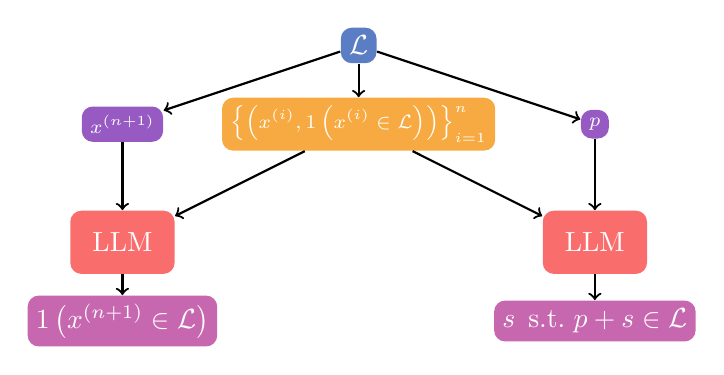
\begin{tikzpicture}
    % Top node with blue background
    \node[fill=customBlue, text=white, rounded corners, inner sep=3pt, baseline] (L) at (0, 0) {$\mathcal{L}$};
    
    % Bottom-left node with purple background (adjusted to align columns)
    \node[fill=customPurple, text=white, rounded corners, inner sep=3pt, baseline] (x) at (-3, -1) {\scriptsize $x^{\left( n + 1 \right)}$};
    
    % Bottom-right node with purple background (adjusted to align columns)
    \node[fill=customPurple, text=white, rounded corners, inner sep=3pt, baseline] (p) at (3, -1) {\scriptsize $p$};
    
    % Bottom-middle node with orange background
    \node[fill=customOrange, text=white, rounded corners, inner sep=3pt, baseline] (data) at (0, -1) {\scriptsize $\left\{ \left( x^{\left( i \right)}, \mathbbm{1} \left( x^{\left( i \right)} \in \mathcal{L} \right) \right) \right\}_{i = 1}^{n}$};
    
    % LLM box below x and data (halfway between them, spaced apart horizontally)
    \node[fill=customRed, text=white, rounded corners, inner sep=8pt, baseline] (LLMx) at (-3, -2.5) {LLM};
    
    % LLM box below p and data (halfway between them, spaced apart horizontally)
    \node[fill=customRed, text=white, rounded corners, inner sep=8pt, baseline] (LLMp) at (3, -2.5) {LLM};
    
    % Box below LLMx with custom magenta background (now under the left LLM box)
    \node[fill=customMagenta, text=white, rounded corners, inner sep=3pt, baseline] (LLMEquation) at (-3, -3.5) {$\mathbbm{1} \left( x^{\left( n + 1 \right)} \in \mathcal{L} \right)$};
    
    % New magenta box on the right with content s t. p + s \in L
    % Adjusted x coordinate to align with LLMp, added dots and more spacing around 'st'
    \node[fill=customMagenta, text=white, rounded corners, inner sep=3pt, baseline] (RightEquation) at (3, -3.5) {$s \, \hspace{3pt} \text{s.t.} \hspace{3pt} p + s \in \mathcal{L}$};
    
    % Drawing original lines (arrows)
    \draw[->, thick] (L) -- (x);
    \draw[->, thick] (L) -- (p);
    \draw[->, thick] (L) -- (data);
    
    % Corrected arrows:
    % - From x to the first LLM box
    % - From data to the first LLM box
    % - From p to the second LLM box
    % - From data to the second LLM box
    \draw[->, thick] (x) -- (LLMx);  % x -> LLMx
    \draw[->, thick] (data) -- (LLMx);  % data -> LLMx
    \draw[->, thick] (p) -- (LLMp);  % p -> LLMp
    \draw[->, thick] (data) -- (LLMp);  % data -> LLMp
    
    % Arrow from LLMx to the new box with the equation
    \draw[->, thick] (LLMx) -- (LLMEquation);  % LLMx -> LLMEquation
    
    % Arrow from LLMp to the new right magenta box with the equation
    \draw[->, thick] (LLMp) -- (RightEquation);  % LLMp -> RightEquation
\end{tikzpicture}

\end{document}
